\subsection{Demo}

\subsubsection{To-do List} \label{todo-list}
Al fine di dare una dimostrazione pratica dell'utilizzo del framework presentato nel paragrafo antecedente, verranno sviluppati due esempi significativi di bubble interattiva.\\
Il primo è una bubble contenente una lista di cose da fare chiamata To-do list.\\
La struttura di questa bubble interattiva sarà analoga a quella presentata nel framework relativamente alla bubble generica e sarà quindi composta da tre parti:
\begin{itemize}
	\item una parte di view tramite la quale l'utente potrà interagire con il sistema, segnando come completate, aggiungendo o rimuovendo voci nella lista;
	\item una parte avente funzione di controller incaricata di ricevere i segnali dall'interfaccia grafica, riconoscerli ed inviarli alla parte di modello in cui verranno gestiti, e viceversa di ricevere i segnali dalla parte di modello e renderizzarli tramite la GUI;
	\item una parte di modello con il compito di gestire la business logic dell'applicativo bubble To-do list.
\end{itemize}
Conformemente a quanto riportato nell'\AnalisiDeiRequisiti{} saranno possibili le seguenti interazioni con il sistema:
\begin{itemize}
	\item creazione di una nuova lista tramite la creazione di una bubble;
	\item aggiunta di elementi alla lista;
	\item rimozione di elementi dalla lista;
	\item possibilità di aggiungere un reminder come notifica.
\end{itemize}

\paragraph{Package To-do list}\mbox{}\\

Il package della To-do List segue il pattern Model-View-Controller (MVC), e dunque contiene i package View, Controller e Model. Il package View contiene tutti gli elementi grafici della To-do List e forma la GUI visibile agli utenti della bubble. Il package Model permette operazioni sui dati riguardanti la To-do List e le notifiche ad essi associate salvati sia nella bubble memory sia nel database attraverso il package Db\-Gateway. Il package Controller è dedicato alla ricezione degli input dagli attori permettendo agli stessi l'interazione con i dati contenuti nel Model e l'aggiornamento della View.

\begin{figure}[H]
	\centering
	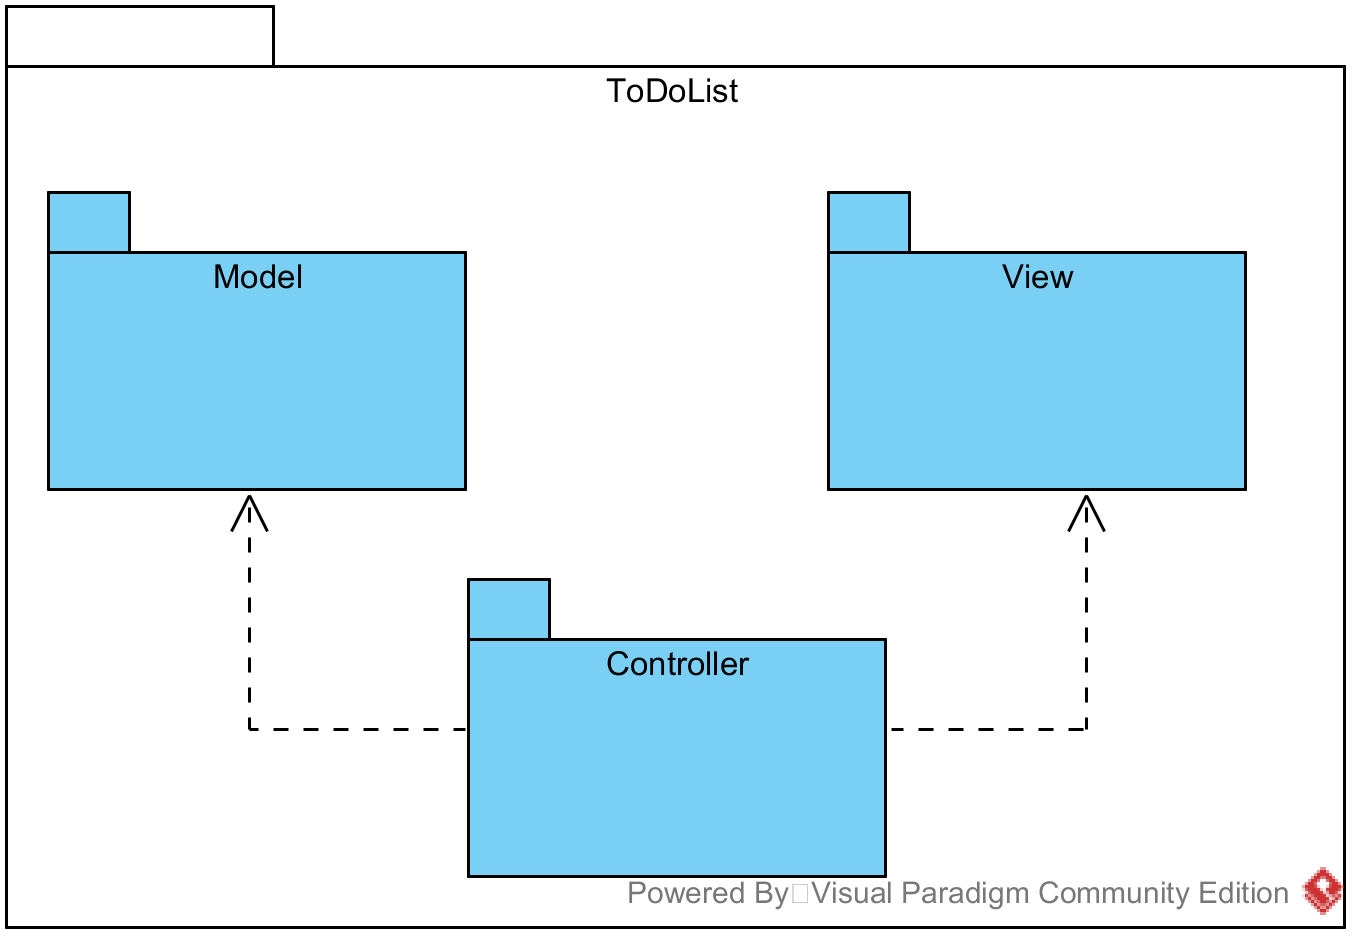
\includegraphics[width=14cm]{../../documenti/SpecificaTecnica/diagrammi_img/classi_e_package/todo.png}
	\caption{Package To-do List}
\end{figure}

\begin{samepage}
\subparagraph{View}\mbox{}\\
\nopagebreak
\begin{figure}[H]
	\centering
	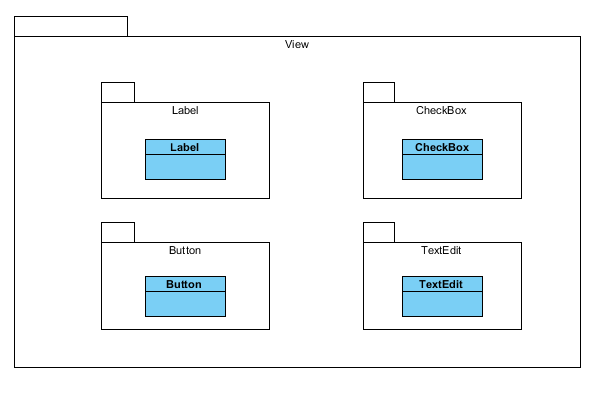
\includegraphics[width=14cm]{../../documenti/SpecificaTecnica/diagrammi_img/classi_e_package/todo_view.png}
	\caption{View}
\end{figure}
\end{samepage}
Le classi presenti in questo package non vengono descritte, in quanto corrispondono a quelle riportate nel framework.

\subparagraph{Model}\mbox{}\\
Il package Model gestisce i dati contenuti nella bubble memory e nel database associato tramite i package BubbleMemory e Db\-Gateway. Permette inoltre di impostare notifiche tramite il package Notification. I dati sono rappresentati dal package List\-Items ovvero le liste contenute nella bubble To-do list. List\-Items\-Container definisce le liste, formate da oggetti della classe List\-Item, cioè singole voci delle liste. 
\begin{figure}[H]
	\centering
	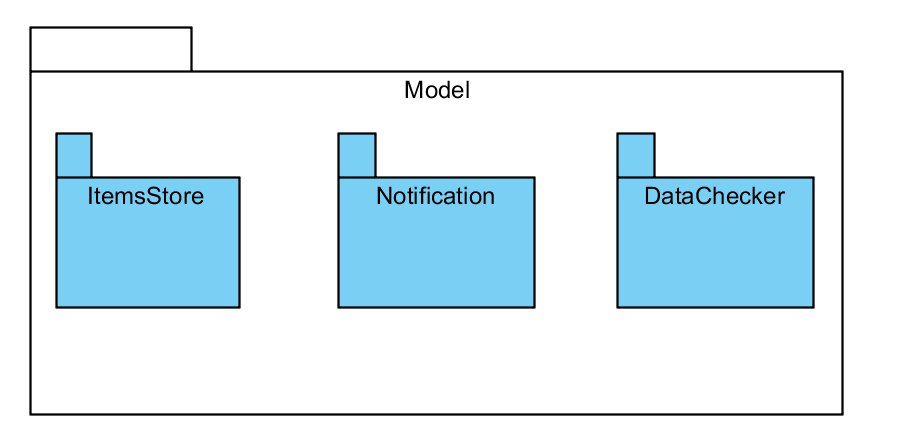
\includegraphics[width=14cm]{../../documenti/SpecificaTecnica/diagrammi_img/classi_e_package/todo_model.png}
	\caption{Model}
\end{figure}

\begin{figure}[H]
	\centering
	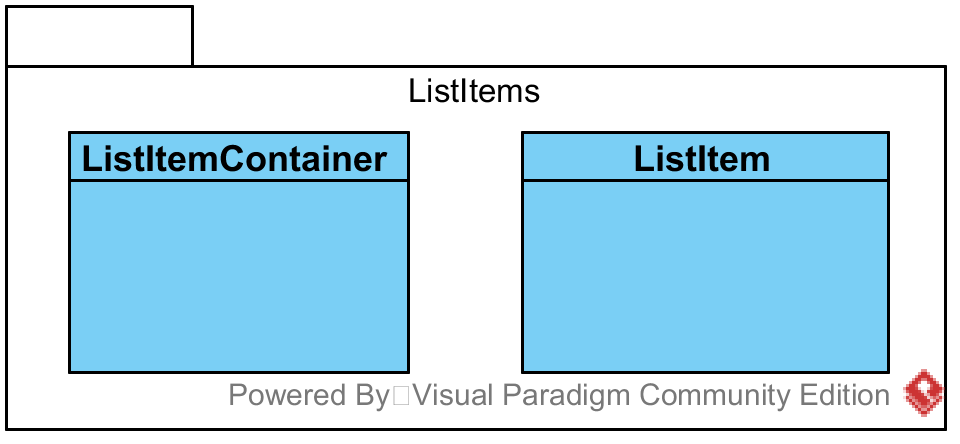
\includegraphics[width=14cm]{../../documenti/SpecificaTecnica/diagrammi_img/classi_e_package/todo_listitems.png}
	\caption{List\-Items}
\end{figure}

\subsubparagraphmark{TodoList\-::Model\-::List\-Items\-::List\-Item}\label{todo-item}\mbox{}\\
\textbf{Descrizione:}\\
La classe List\-Item rappresenta un'entrata per la To-do list.\\
\textbf{Utilizzo:}\\
L'utilizzo di questa classe è quello di fornire un'implementazione per le entrate della bubble To-do list in modo da poter creare o eliminare voci dalla lista, essere segnate come completate o settare un reminder.\\

\subsubparagraphmark{TodoList\-::Model\-::List\-Items\-::List\-Item\-Container}\label{todo-container}\mbox{}\\
\textbf{Descrizione:}\\
La classe List\-Item permette la gestione di una collezione di voci della To-do list definite dalla classe List\-Item.\\
\textbf{Utilizzo:}\\
Questa classe offre la possibilità di aggiungere, rimuovere e restituire elementi da una collezione di elementi della To-do list.\\


\subsubparagraphmark{TodoList\-::Model\-::Db\-Gateway\-::Data\-Checker}\label{todo-gateway}\mbox{}\\
\textbf{Descrizione:}\\
La classe Db\-Gateway verifica la correttezza dei dati rispetto ad uno schema dato.
\textbf{Utilizzo:}\\
Questa classe permette di verificare l'integrità dei dati inviati dall'utente rispetto ad uno schema dato.

\subparagraph{Controller}\mbox{}
\begin{samepage}
	\subsubparagraphmark{TodoList\-::Controller\-::Todo\-Controller}\label{todo-controller}\mbox{}\\
	\nopagebreak
	\begin{figure}[H]
		\centering
		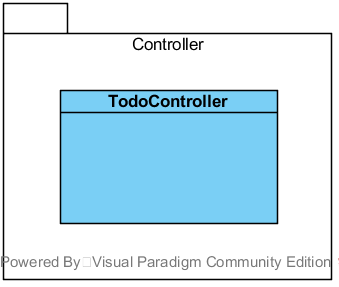
\includegraphics[height=5cm]{diagrammi_img/classi_e_package/todo_controller}
		\caption{Controller\-::Todo\-Controller}
	\end{figure}
\end{samepage}
\textbf{Descrizione:}\\
La classe TodoController svolge il ruolo di controller all'interno della bubble To-do list. \\
\textbf{Utilizzo:}\\
Viene utilizzata per controllare le interazioni tra GUI e model all'interno della bubble. Corrisponde alla GenericBubble del framework. \\